
%--------------------------------------------------------------
% ĐẠI HỌC BÁCH KHOA HÀ NỘI
% Trường Điện - Điện tử
% Khoa Điện
%
% MẪU SOẠN THẢO ĐỒ ÁN
%--------------------------------------------------------------



\documentclass{thesis}

\usepackage[utf8]{inputenc} % 
\usepackage[T5]{fontenc} % Font Vietnamese
\usepackage{subcaption}
\usepackage{subfig}
\usepackage{graphicx} % Figure
\usepackage{hyperref}
\usepackage{amsmath}
\usepackage{amsfonts}
\usepackage{titlesec}
\newcommand{\centeredappendixtitle}[1]{\titleformat{\section}[display]{\filcenter\normalfont\Large\bfseries}{#1}{1ex}{}}

\usepackage{tabularx}
%\usepackage{amsmath}
\usepackage{longtable}
\usepackage{pdfpages}
\usepackage{float} % Set position figure or table
\usepackage{url}
\usepackage{mathptmx} % select font Times New Roman
\usepackage{geometry} % Set parameters paper
\usepackage{xcolor}
\usepackage{multirow}
\usepackage{mathptmx}
\usepackage{xurl} 
\usepackage[fontsize=13pt]{scrextend} % set font size = 13pt
\usepackage{indentfirst} % Indent first line
\usepackage{changepage}
\usepackage{afterpage}
\usepackage{booktabs}
\usepackage{setspace}

%% START DOCUMENT
\begin{document}
\sloppy
% CREATE COVER PAGE

\begin{center}
    \vspace{12pt} % line spacing
        \textbf{\fontsize{15pt}{0pt} \selectfont{}HANOI UNIVERSITY OF SCIENCE AND TECHNOLOGY \\ \vspace{3pt} SCHOOL OF ELECTRICAL AND ELECTRONIC ENGINEERING}
    \vspace{0.5cm}
    
% INSERT LOGO
\begin{figure}[H]
    \centering
    
\includegraphics[width=3cm,height=4cm]{logoBK.png}
\end{figure}

% THESIS TYPE
\vspace{48pt}
        \fontsize{25pt}{0pt}\selectfont{} \textbf{PROJECT I}
\vspace{24pt}

 % THESIS TITTLE
        \textbf{\fontsize{17pt}{0pt}\selectfont{}Public Electric Vehicle Charging: \\
        A Comprehensive Review}
    \vspace{18pt}

% NAME
        \fontsize{14pt}{0pt}\selectfont{} \textbf{Dao Quoc Khanh}
    \vspace{3pt}

% EMAIL    
        \fontsize{14pt}{0pt}\selectfont{} Khanh.DQ222725@sis.hust.edu.vn
    \vspace{12pt} % line spacing

% MAJOR
        \fontsize{14pt}{0pt}\selectfont{} \textbf{Advanced Program: \\
        Power Systems and Renewable Energy}  
\end{center}
    \vspace{48pt}

% INFORMATION: SUPERVISOR NAME, STUDENT NAME,...
\begin{table}[H]
    \centering
        \begin{tabular}{l l c}
            \textbf{Instructor:}    & Assoc. Prof Nguyen Duc Tuyen \vspace{6pt} &  \\ 
            &\vspace{3pt} & \fontsize{10pt}{0pt}\selectfont{} Signature of Instructor \\
            \textbf{Department:} & Electrical Engineering \vspace{3pt}\\ 
            \textbf{School:} & Electrical \& Electronic Engineering
        \end{tabular}
\end{table}

% TIME
\begin{center}
    \vspace{48pt}
    \fontsize{14pt}{0pt}\selectfont{} Ha Noi, 1/2025
\end{center}

% CREATE A NEW PAGE AND REMOVE PAGE NUMBER
%\thispagestyle{empty}
  %  \newpage
  %      \clearpage
            \thispagestyle{empty}
                \cleardoublepage

\thispagestyle{empty}
    \clearpage
        \thispagestyle{empty}
        
%SUMMARY PART 
\section*{ABSTRACT}
    \thispagestyle{empty}
Most vehicles worldwide rely on fossil fuels, leading to the release of harmful gases, for example $CO_2$, $CO$, $NO_x$, and other fine dust particles. To reduce emissions in the transportation sector, Electric Vehicles (EVs) have gained significant attention. They are considered a promising alternative to gasoline-powered vehicles, due to their advantages of zero direct carbon dioxide emissions, higher energy efficiency, and reduced noise pollution. Many countries have implemented policies to promote EV adoption, aiming to reduce overall emissions through both legal and economic incentives. To meet the escalating demand for electric vehicles, nations must correspondingly develop robust charging infrastructure, with classifications will be included in this report. However, the large-scale deployment of charging stations will significantly stress the power distribution system, potentially causing voltage and frequency instability and increasing the risk of grid overload. Managing EV charging/discharging via controlled charging process or Vehicle-to-Grid (V2G) technology (allowing EVs to both draw and supply power) can help stabilize the grid. Furthermore, if the grid still depends on fossil fuels generation, EV charging still produces substantial emissions. Therefore, integrating renewable energy sources with energy storage into charging stations is being explored to provide clean power, thus enhancing EV sustainability and supporting grid stability. Through a review of existing literature, the negative effects of EV charging stations (EVCSs) on the power grid and potential solutions can be assessed. Finally, conclusions and recommendations will be presented.
\thispagestyle{empty}
    \clearpage

 % CONTENT
\tableofcontents 
    \thispagestyle{empty}
        \newpage
            \thispagestyle{empty}

% LIST OF SYMBOLS AND ABBREVIATIONS
\pagenumbering{roman}   % Roman numbering: i, ii, iii, iv,...
\section*{LIST OF ABBREVIATIONS}
    \phantomsection \addcontentsline{toc}{section}{\numberline{} LIST OF ABBREVIATIONS}

% Create table
    \begin{tabular}{ l l }
    \hspace{1cm} AC & \hspace{2cm} Alternating Current \\
    \hspace{1cm} APS & \hspace{2cm} Announced Pledges Scenario \\
    \hspace{1cm} BESS & \hspace{2cm} Battery Energy Storage System \\
    \hspace{1cm} DC & \hspace{2cm} Direct Current \\
    \hspace{1cm} EV & \hspace{2cm} Electric Vehicle \\
    \hspace{1cm} EVCS & \hspace{2cm} Electric Vehicle Charging Station \\
    \hspace{1cm} IEA & \hspace{2cm} International Energy Agency \\
    \hspace{1cm} IEEE & \hspace{2cm} Institute of Electrical and Electronics Engineers \\
    \hspace{1cm} LCOE & \hspace{2cm} Levelized Cost of Energy \\
    \hspace{1cm} LDV & \hspace{2cm} Light-duty Vehicle \\
    \hspace{1cm} NPV & \hspace{2cm} Net Present Value \\
    \hspace{1cm} NZE & \hspace{2cm} Net Zero Emissions by 2050 Scenario \\
    \hspace{1cm} PV & \hspace{2cm} Photovoltaic \\
    \hspace{1cm} RES & \hspace{2cm} Renewable Energy Sources \\
    \hspace{1cm} SOC & \hspace{2cm} State of Charge \\
    \hspace{1cm} STEPS & \hspace{2cm} Stated Policies Scenario \\
    \hspace{1cm} WPT & \hspace{2cm} Wireless Power Transfer \\
    \hspace{1cm} WT & \hspace{2cm} Wind Turbine \\

    
\end{tabular}  
    \newpage

% LIST OF FIGURES
{\let\oldnumberline\numberline
    \renewcommand{\numberline}{Figure~\oldnumberline}
        \listoffigures}
            \phantomsection\addcontentsline{toc}{section}{\numberline{} LIST OF FIGURES}
\newpage

% LIST OF TABLES
{\let\oldnumberline\numberline
    \renewcommand{\numberline}{Table~\oldnumberline}
        \listoftables}
            \phantomsection\addcontentsline{toc}{section}{\numberline{} LIST OF TABLES}
\newpage

%% --------------------------------------------------%%
%------------CHAPTER 1---------------------------%
%%-----------------------------------------------------%

\pagenumbering{arabic} % numbering: 1,2,3,...
    \section*{CHAPTER 1. INTRODUCTION} 
        \addcontentsline{toc}{section}{\numberline{}CHAPTER 1. INTRODUCTION} % Reference to content

\setcounter{section}{1} 
    \setcounter{subsection}{0}
        \setcounter{figure}{0}
            \setcounter{table}{0}
%%--------------------------------------------------------

The rising demand for energy and the impacts of climate change, such as extreme weather, have degraded quality of life and threatened ecosystems, increasing public awareness of environmental challenges. Reducing greenhouse gas (GHG) emissions is essential for global net-zero goals, with transportation being the second-largest CO2 source in Europe and the largest in the U.S. \cite{VanFan2018}. Electric vehicles (EVs), which produce no direct carbon emissions and are nearly twice as energy-efficient as gasoline cars, offer a key solution. Driven by strong policies, global EV registrations reached 14 million in 2023, nearly six times the 2018 total \cite{global_ev_outlook_2024}.

Home charging is currently the most common method for electric car owners, with nearly ten times as many private chargers as public ones (Fig. \ref{fig:public_private}). Convenient overnight charging at home often leverages lower electricity prices during off-peak hours. However, access to home charging varies significantly by region, influenced by urban density, population type, and income levels. In densely populated cities, where multi-unit dwellings are prevalent, EV owners often rely more heavily on public charging, as seen in Korea, which has the world's highest ratio of public charging capacity to EVs \cite{global_ev_outlook_2024}.

\begin{figure}[h!]
\captionsetup{font=footnotesize}
\captionsetup{justification=centering}
    \centering
    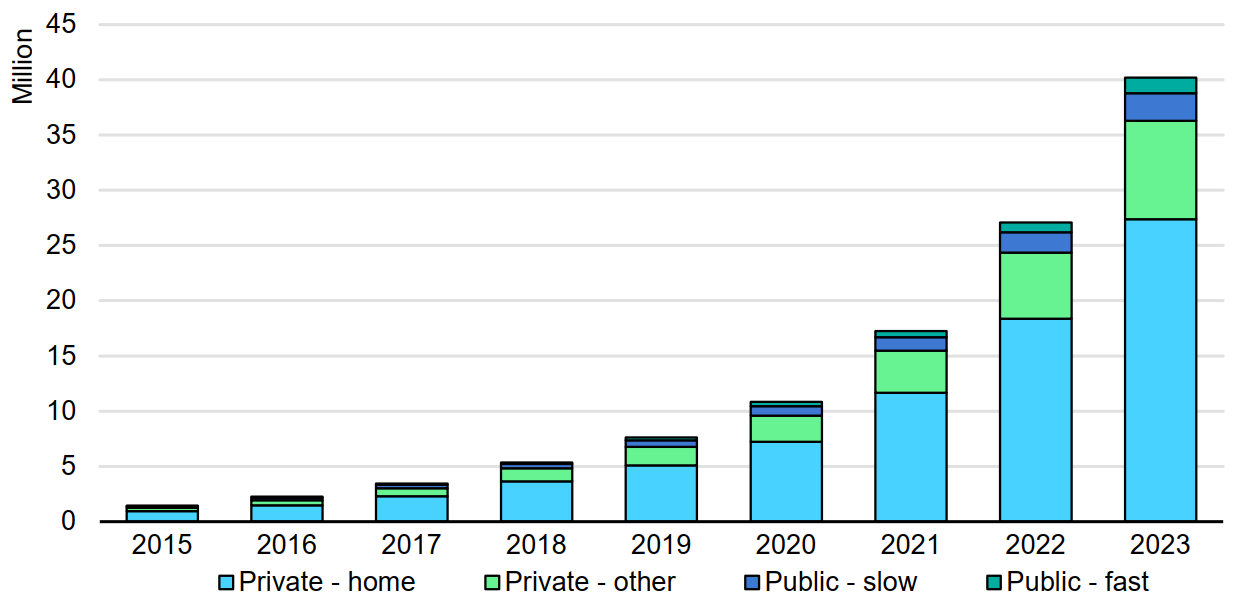
\includegraphics[width=1\textwidth]{FIGURES/Chapter 1/Installed public and private light-duty vehicle charging points by power rating (public) and by type (private), 2015-2023.png}
    \caption{Installed public and private light-duty vehicle charging points by power rating (public) and by type (private), 2015-2023.}
    \label{fig:public_private}
    \cite{global_ev_outlook_2024}
\end{figure}

As the number of EVs increases and home charging times remain slow, the need for faster public charging services becomes unavoidable. Furthermore, typical home electrical systems cannot handle the large power demands required for rapid EV charging. Consequently, the development of public electric vehicle charging stations (EVCSs) is crucial. However, this development presents challenges, including substantial land use, high power demand, and potential grid impacts. These charging infrastructures are essential due to the increasing integration of EVs into the electrical grid, which, while currently contributing a small portion of overall energy consumption, will significantly grow as EV adoption expands. Moreover, EVs interact with the grid as flexible loads, with the potential to supply power via Vehicle-to-Grid (V2G) technology. Their impact on the electrical system includes various aspects such as charging station types, harmonic distortions, voltage fluctuations in distribution networks during charging, and economic effects from the charging process, as well as their potential to provide grid ancillary services through integrated energy storage systems and renewable energy sources.

The rest of the report is structured as follows:
\begin{itemize}
    \item \textbf{Chapter 2. EV charging methods, technologies and classifications.} This chapter is about classifications of different charging methods depends on several criteria, and their related standards
    \item \textbf{Chapter 3. Impacts of Electric Vehicles on the distribution grid.} Negative impacts of charging EVs to the grid is analyzed in this section
    \item \textbf{Chapter 4. Strategies and solutions to mitigate the effects of EVs on the power grid.} List of studies have been found solutions to achieve one or more objective simultaneously
    \item \textbf{Chapter 5. Conclusion.} Conclusion and recommendations for improvements in EV charging protocols and infrastructures
\end{itemize}

\newpage

%%-------------------------------------------------------%%
% --------------------------------------------------------%
%---------------------------------------------------------%

%---------------------------------------------------------%%
%% ----------CHAPTER 2 -------------------%%
%---------------------------------------------------------%%
\section*{CHAPTER 2. EV CHARGING METHODS, TECHNOLOGIES AND CLASSIFICATIONS}
\label{chuong2}
    \addcontentsline{toc}{section}{\numberline{}CHAPTER 2. EV CHARGING METHODS, TECHNOLOGIES AND CLASSIFICATIONS}

\setcounter{section}{2} 
    \setcounter{subsection}{0}
        \setcounter{figure}{0}
            \setcounter{table}{0}

EV charging technologies and methods have advanced significantly to address the growing demand for efficient and convenient charging solutions. These advan-cements have led to diverse classifications of EV charging infrastructure based on factors such as location, available power sources (e.g., RES, BESS, and conventional sources), charging speed, power transfer method, purpose, and more. In terms of their connection to the electric vehicle, charging technologies are classified into three categories based on: wired, wireless, and battery exchange. These classifications are illustrated in Fig. \ref{fig:Charging Methods} \cite{EVCM}. The terms "EV charger" and "charging station" are often used interchangeably but can have nuanced differences in the context of electric vehicles and their infrastructure \cite{28_in_EVCM}. Both systems can derive power from various energy sources, such as the grid, RES, BESS, or hybrid systems, utilizing either line-frequency transformers (LFT) or modern solid-state transformers (SST) coupled with power-electronics-based conversion units \cite{29_in_EVCM}.

\begin{figure}[h!]
\captionsetup{font=footnotesize}
\captionsetup{justification=centering}
    \centering
    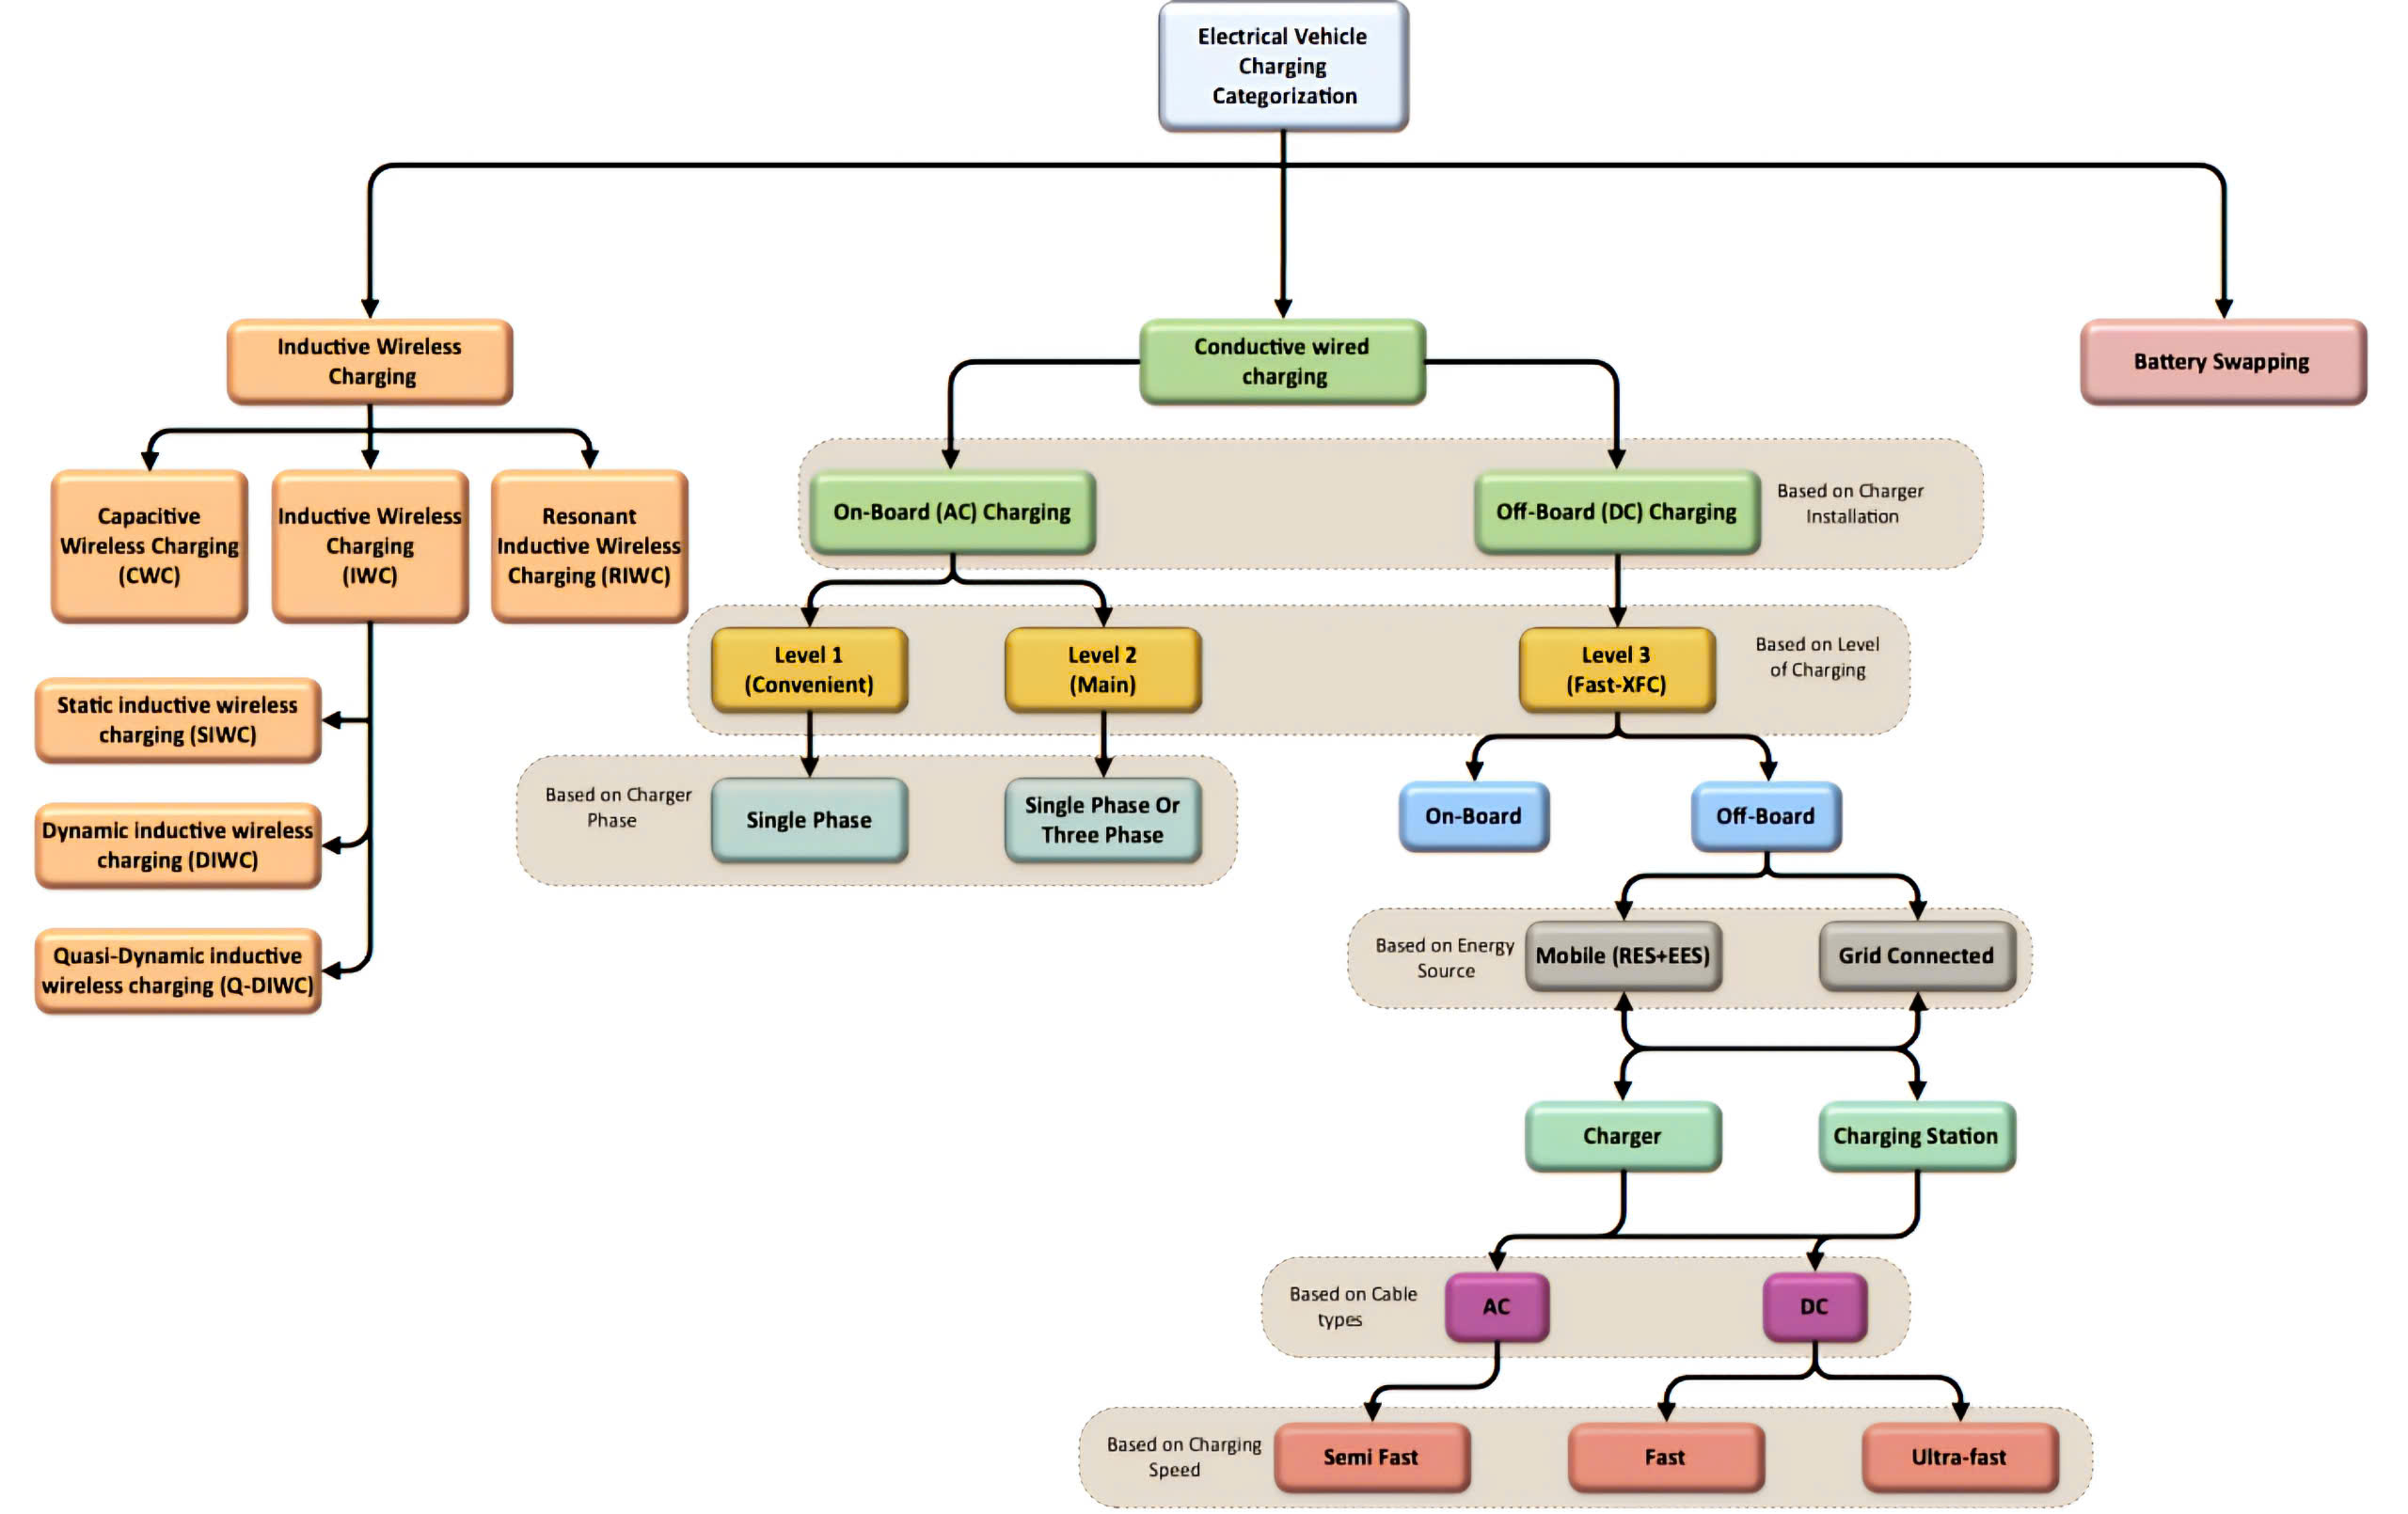
\includegraphics[width=1\textwidth]{FIGURES/Chapter 2/charging methods.jpg}
    \caption{Detailed Categorization of EVs charging technologies, modes, and methods}
    \label{fig:Charging Methods}
    \cite{EVCM}
\end{figure}

An EV charger typically refers to a single unit capable of charging one vehicle at a time, as depicted in Fig. \ref{fig:Charging Config} \cite{EVCM}. Conversely, a charging station is a broader term encompassing multiple EV chargers alongside the necessary electrical connections and safety features to ensure reliable charging. Charging stations are commonly installed in diverse locations, including public parking lots, shopping centers, highways, workplaces, and residential areas.

\begin{figure}[h!]
\captionsetup{font=footnotesize}
\captionsetup{justification=centering}
    \centering
    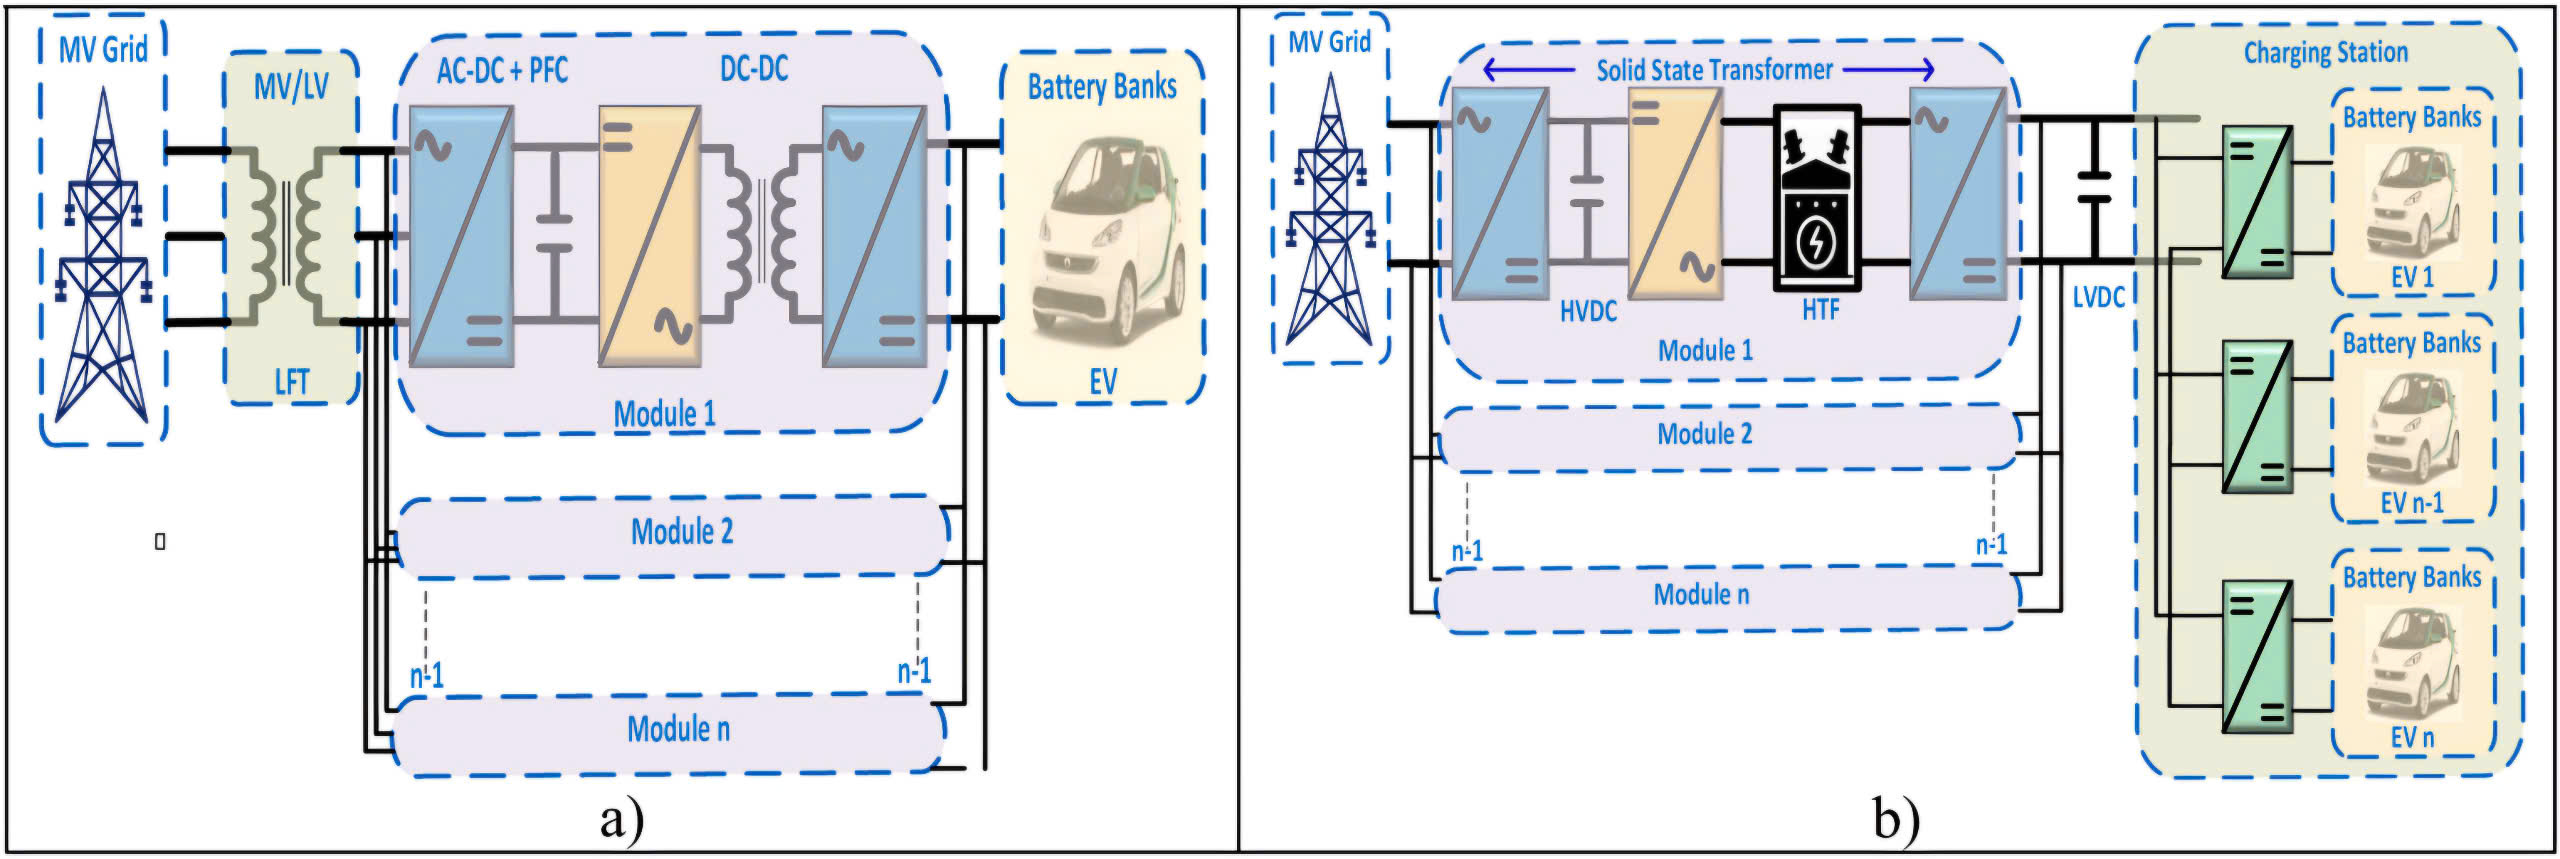
\includegraphics[width=1\textwidth]{FIGURES/Chapter 2/charging config.jpg}
    \caption{(a) Configuration for a charger using LFT; (b) Configuration for a charging station using SST}
    \label{fig:Charging Config}
\end{figure}

The primary methods for recharging electric vehicles include conductive char-ging, wireless charging, and battery swapping, as shown in Fig. \ref{fig:Charging Methods}. Conductive charging employs a cable to connect the power source directly to the vehicle's battery. Wireless charging, in contrast, achieves energy transfer without a physical connection. Battery swapping replaces a depleted battery with a fully charged one. Among these, conductive charging is the most prevalent method due to its maturity and accessibility. This method involves physically connecting a cable to the vehicle’s charging port, enabling electricity to flow from the power source to the vehicle’s battery. While future advancements in technology and infrastructure may shift the balance between these methods, conductive charging remains the most widely adopted approach today \cite{32_in_EVCM}. 

\subsection{Conductive charging}
Beside charging in one direction from the grid to the EVs, conductive char-ging also provisions vehicle-to-grid (V2G) facility to reduce grid loss, regulate voltage, boost active power, and reduce reactive power. Fig. \ref{fig:wired charging} illustrates visual representations of the conductive charging system.
\begin{figure}[h!]
\captionsetup{font=footnotesize}
\captionsetup{justification=centering}
    \centering
    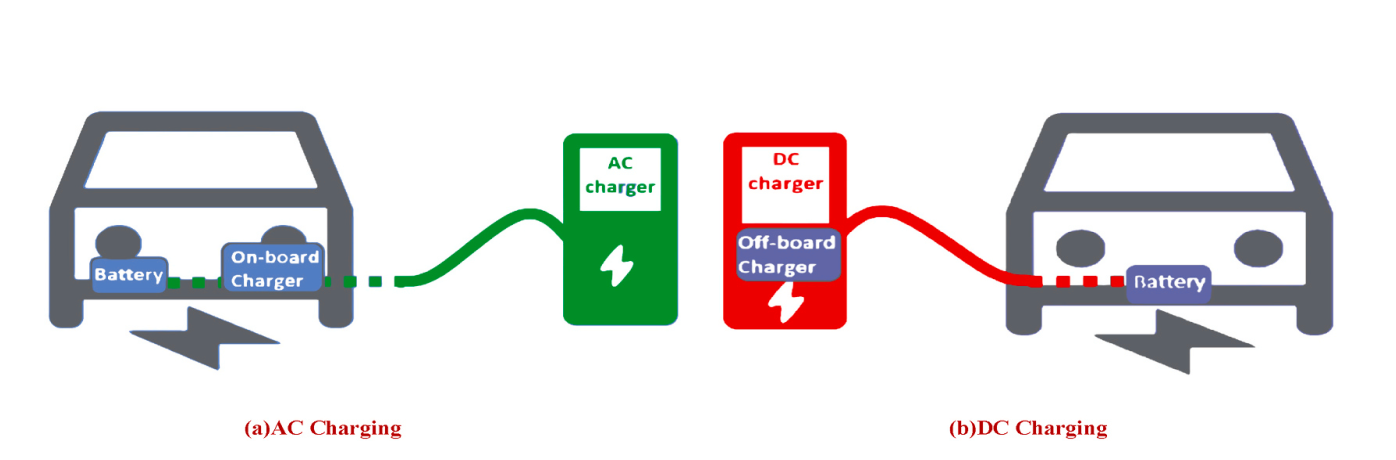
\includegraphics[width=1\textwidth]{FIGURES/Chapter 2/Wired Charging Illustration.png}
    \caption{Conductive charging illustration}
    \cite{charging_types}
    \label{fig:wired charging}
\end{figure}
The operations of both Uni-directional and Bi-directional chargers are as follows \cite{charging_types}:
\begin{itemize}
    \item \textit{i. Operation of an Uni-Directional Battery Charger:} Diode bridge rectifiers (DBR), filter stages, and DC-DC converters are all included in uni-directional chargers. The DBR can be single-phase or three-phase to boost charging power. Additionally, isolation is ensured during EV charging by using a high-frequency isolation transformer. The above converter topology cannot inject energy from an EV battery into the utility grid. Providing reactive power to or from the primary electrical grid without draining EV batteries enables auxiliary services, particularly voltage regulation. Uni-directional battery chargers offer a simple, cost-effective, and safe method for managing EV deployments. As a result, the power grid needs topologies that allow EVs to operate as a form of distributed energy storage. The 1- Ø uni-directional on-BC is depicted in Fig. \ref{fig:1 phase}. 
    \begin{figure}[h!]
        \captionsetup{font=footnotesize}
        \captionsetup{justification=centering}
        \centering
        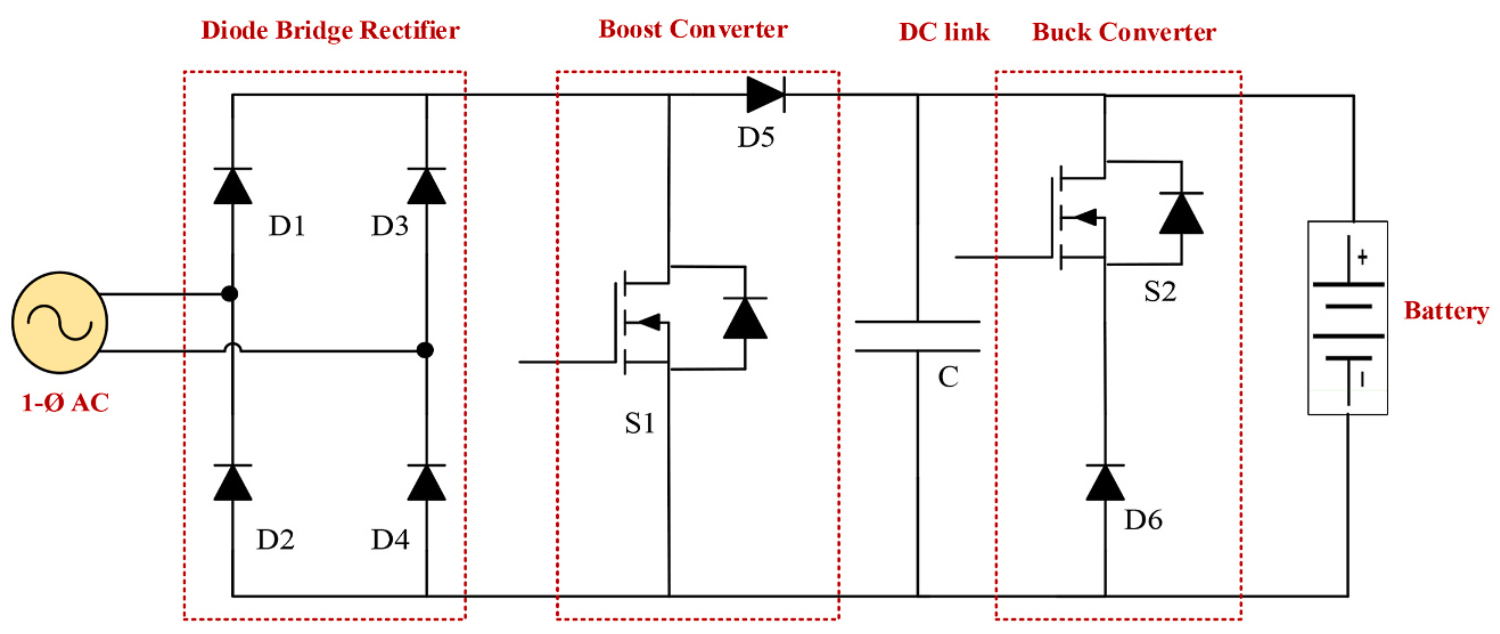
\includegraphics[width=1\textwidth]{FIGURES/Chapter 2/1- Ø Uni-directional on-BC.png}
        \caption{1- Ø Uni-directional on-BC}
        \label{fig:1 phase}
    \end{figure}
    \item \textit{ii. Operation of a Bi-Directional Battery Charger:} The two main parts of a bi-directional EV charger are a DC-DC converter and an active front end (AFE) that can be single or three phases. AFE is a bi-directional AC-DC converter that regulates DC bus voltage, controls quasi-sinusoidal grid currents, and maintains a unity power factor reactive power exchange with the grid. During the second stage, it is possible to regulate the battery’s charging current. Depending on the circuit arrangement, the DC-DC converter might be isolated. The two main parts of a bi-directional EV charger are a DC-DC converter and an active front end (AFE) that can be single or three phases. Fig. \ref{fig:3 phase} illustrates the 3- Ø bi-directional on-BC.
    \begin{figure}[h!]
        \captionsetup{font=footnotesize}
        \captionsetup{justification=centering}
        \centering
        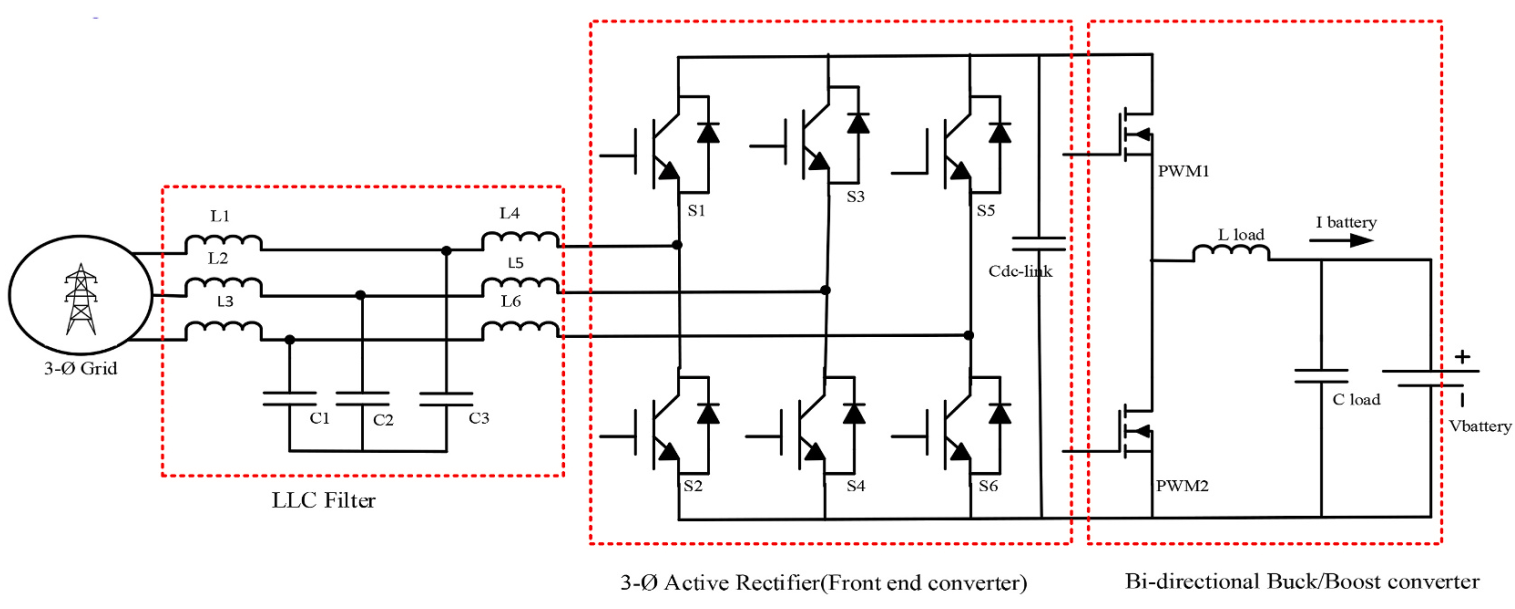
\includegraphics[width=1\textwidth]{FIGURES/Chapter 2/3- Ø Bi-directional off-BC.png}
        \caption{3- Ø Bi-directional off-BC}
        \label{fig:3 phase}
    \end{figure}
\end{itemize}

The following outlines the typical procedure for a conductive battery charger to replenish a battery's charge \cite{charging_types}:
\begin{itemize}
    \item Initially, a battery charger performs rectification and conditioning of the grid power to make it suitable for battery charging.
    \item Subsequently, depending on the specific requirements, a collection of power electronic converters, such as AC-to-DC rectifiers, DC-to-AC inverters, or DC-to-DC choppers, modify the charger's input power. These chargers are further classified by their number of conversion stages, such as single-stage, two-stage, and so on.
   \item A single-stage approach is generally inadequate for battery chargers used in automotive applications due to the high power demand, the need for rapid charging methodologies, and limitations imposed by grid power factor regulations. Therefore, chargers involve a multi-stage conversion process. This involves several steps, including alternating current (AC) rectification, power factor correction (PFC), conversion of direct current (DC) to alternating current (AC) at a high frequency, galvanic isolation, rectification again, and lastly, a DC-DC conversion to achieve the desired charging profile.
\end{itemize}

Conductive chargers can be further classified based on installation type: on-board (AC) or off-board (DC).

\subsubsection{AC charging}
On-board AC chargers draw power from the grid, which is routed through a charging station to the vehicle via an embedded AC-DC rectifier. These chargers, typically used in residential and public parking infrastructures, are limited to Levels 1 and 2 under the charging classification system \cite{33_in_EVCM}. On-board chargers offer advantages such as cost-effectiveness (ranging from \$625 to \$3750), simplicity, and enhanced security since they are embedded in the vehicle. However, they are constrained by vehicle size and power availability, typically capped at 20–40 A and 6–8 kW, resulting in charging times of no less than six hours \cite{31_in_EVCM}.

\subsubsection{DC charging}
Off-board DC fast chargers, on the other hand, rely on power electronics, including AC-DC rectifiers and DC-DC converters, to deliver rapid charging. These systems are more expensive (ranging from \$37,500 to \$200,000) due to their complex infrastructure, larger size, and higher power demands—often double that of household consumption. Despite these challenges, they provide significant benefits, such as reduced charging times (as low as 10 minutes depending on infrastructure) and the ability to handle currents up to 250 A and power levels ranging from 20–350 kW under Level 3 classifications. Systems exceeding 350 kW and 400 A fall under extreme fast charging (XFS) \cite{34_in_EVCM}.

The categorization of EV charging levels varies across studies, with one study \cite{28_in_EVCM} identifying four levels of charging (see Table \ref{tbl:4lvcharging}) \cite{EVCM}. Detailed comparisons between AC/DC chargers and on-board/off-board systems are presented in \cite{32_in_EVCM,34_in_EVCM}.

\begin{table}[h!]
\centering
\captionsetup{font=footnotesize}
\captionsetup{justification=centering}
\caption{Four-level charging load of EVs}
\small
\begin{tabular}{@{}lllll@{}}
\hline
\toprule
\begin{tabular}[c]{@{}l@{}} \textbf{Type} \end{tabular} &
\begin{tabular}[c]{@{}l@{}} \textbf{Voltage} \end{tabular} &
\begin{tabular}[c]{@{}l@{}} \textbf{Maximum} \\ \textbf{power (kW)}
\end{tabular} &
\begin{tabular}[c]{@{}l@{}} \textbf{Charging} \\ \textbf{time (h)}\end{tabular} &
\begin{tabular}[c]{@{}l@{}} \textbf{Standard} \end{tabular} \\
\midrule
Level 1 & 120 US (AC) & 1.9 & 4--11 &  SAE J1772 \\
\textit{(Slow)} & 230 EU (AC) & 7.4 & 11--36 & IEC 62196--2 (Mennekes)  \\ \midrule
Level 2 & 240 US (AC) & 19.2 & 2--6 &  SAE J1772 \\ 
\textit{(Semi-fast)} & 400 EU (AC) & 43 & 2--3 & IEC 62196--2 (Mennekes)
\\ \midrule
Level 3 & 208--600 (DC) & 50--350 & 0.16--0.5 & SAE J1772, CCS, 
\\ \textit{(Fast)} & & & & CHAdeMO, Tesla
\\ \midrule
Level 4 & $\geq 800$ (DC) & >400 & $\sim$ gas \\
\textit{(Ultra-fast)} & & & refueling
\\ \bottomrule
\end{tabular}
\label{tbl:4lvcharging}
\end{table}

EV charging infrastructure is guided by international standards. In Europe, the International Electrotechnical Commission (IEC) standards are prevalent, while in the United States, SAE and IEEE standards are commonly employed. These standards classify charging systems based on factors such as charging time, power levels, and vehicle technologies. Among the most widely adopted are IEC 61851 and SAE J1772, which share similarities but differ in terminology; SAE uses "level" to describe output intensity, while IEC prefers the term "mode" \cite{35_in_EVCM,36_in_EVCM}. Table \ref{tbl:diffEVcharging} provides an overview of various EV charging levels and standards based on recent literature \cite{EVCM}.

\begin{table}[h!]
\centering
\captionsetup{font=footnotesize}
\captionsetup{justification=centering}
\caption{Different EV charging installations, levels, and standards}
\scriptsize
\begin{tabular}{@{}lllllll@{}}
\hline
\toprule
\begin{tabular}[c]{@{}l@{}} \textbf{Charger} \\ \textbf{installation}\end{tabular} & 
\begin{tabular}[c]{@{}l@{}} \textbf{Charger} \\ \textbf{phase}\end{tabular} & 
\begin{tabular}[c]{@{}l@{}} \textbf{Voltage} \\ \textbf{(V)}\end{tabular} & 
\begin{tabular}[c]{@{}l@{}} \textbf{Current} \\ \textbf{(A)}\end{tabular} & 
\begin{tabular}[c]{@{}l@{}} \textbf{Supply} \\ \textbf{interface}\end{tabular} & 
\begin{tabular}[c]{@{}l@{}} \textbf{Charging} \\ \textbf{time}\end{tabular} & 
\begin{tabular}[c]{@{}l@{}} \textbf{Standard}\end{tabular} \\ 
\midrule
\multirow{2}{*}{On-board} & 1-Ø & 120/230 & 12--16 & Residential & 20 & SAE J1772 \cite{37_in_EVCM} \\ 
                          & 1-Ø & 120/230 & 20 & Residential & 11 & SAE J1772 \cite{38_in_EVCM} \\ 
\midrule
\multirow{2}{*}{On-board} & 1-Ø or 3-Ø & 240 & 32 & Dedicated EVSE & 7--10 & IEC 61,851 \cite{39_in_EVCM} \\ 
                          & 1-Ø or Split-Ø & 208/240 & 12--80 & Private and commercial & 5 & IEC 62196--2 \cite{40_in_EVCM} \\ 
\midrule
\multirow{3}{*}{Off-board} & 1-Ø or 3-Ø & 240 & 32 & Publicly charging & 2--6 & SAE J1772 \cite{41_in_EVCM} \\ 
                           & 3-Ø & 480 & 250 & Dedicated EVSE & 30 min & IEC 61851 \\ 
                           & 3-Ø & 240 & 250--500 & Commercial & 30 min & IEC 61851--23 \cite{43_in_EVCM} \\ 
\midrule
\multirow{3}{*}{Off-board} & 3-Ø & 208--600 & 300 & Refueling stations & 12--30 min & SAE J1772 \cite{30_in_EVCM} \\ 
                           & 3-Ø & 800--1000 & 400 & Dedicated EVSE & 12--30 min & IEC 61851 \\ 
                           & Higher Polyphase & 1000 & 400 & Commercial & 5 min & SAE J2847/2 \cite{43_in_EVCM} \\ 
\bottomrule
\end{tabular}
\label{tbl:diffEVcharging}
\end{table}

\subsection{Wireless charging}
Wireless power transfer (WPT) systems, particularly for electric vehicle (EV) charging, operate based on Faraday's law of electromagnetic induction. Inductive charging, a form of contactless magnetic power transfer, facilitates EV charging wirelessly. These systems, which can be stationary or dynamic, are typically utilized in static locations like parking lots, garages, or at traffic signals. Several automakers, including Nissan, Chevrolet, Audi, Toyota, and Mitsubishi, have developed or are developing WPT systems for their EV models through collaborations with companies like Evatran, Delphi, and WiTricity \cite{charging_types}. Fig. \ref{fig:WCI} illustrates visual representations of the wireless charging system.

\begin{figure}[h!]
    \captionsetup{font=footnotesize}
    \captionsetup{justification=centering}
    \centering
    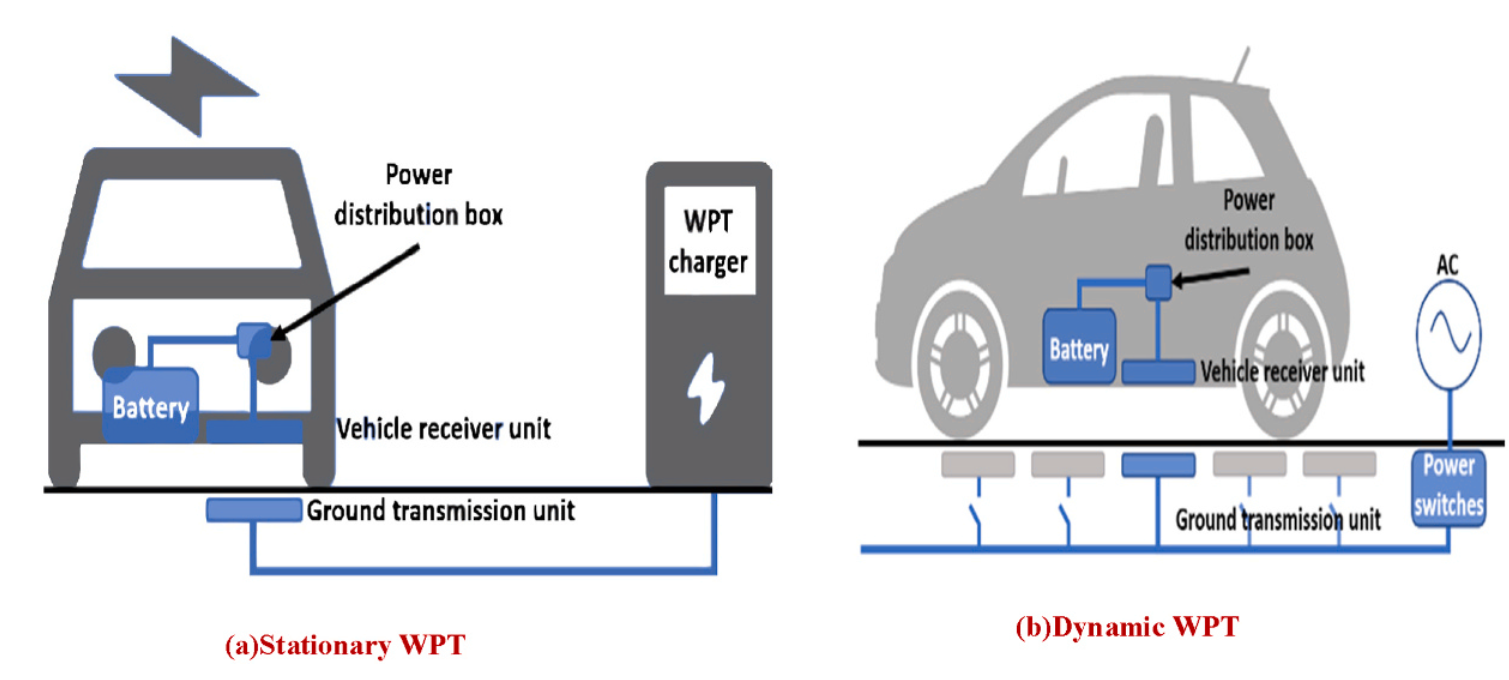
\includegraphics[width=1\textwidth]{FIGURES/Chapter 2/Wireless charging Illustrations.png}
    \caption{Wireless charging illustrations}
    \label{fig:WCI}
\end{figure}

Electromagnetic induction has broad applications for wireless power delivery, including use in automobiles, personal care devices, and healthcare products. Induc-tive charging, which derives its name from energy transmission via inductive coupling, uses an alternating current in a charging station's inductive coil. This current flow generates a time-varying magnetic field, which in turn induces a current in the receiving device's induction coil. This induced current is then converted to direct current (DC) to charge the battery. The structure of a wireless power transfer system for EV is illustrated in Fig. \ref{fig:WPT}.

\begin{figure}[h!]
    \captionsetup{font=footnotesize}
    \captionsetup{justification=centering}
    \centering
    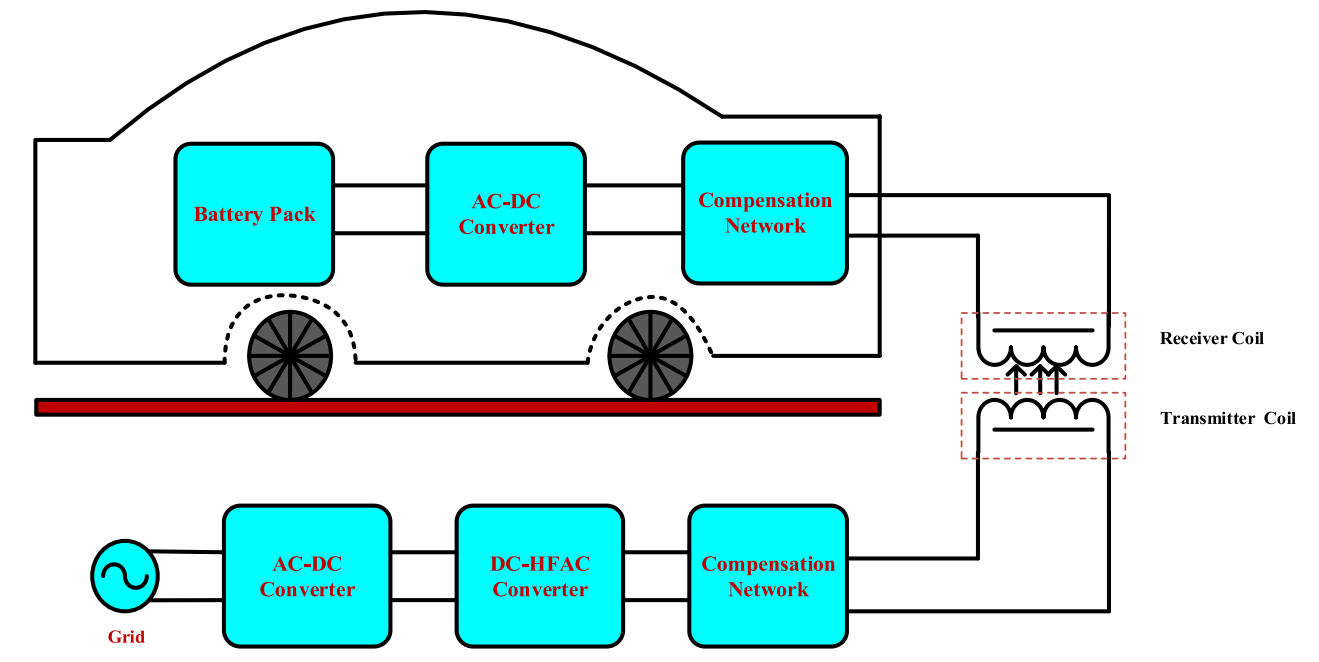
\includegraphics[width=1\textwidth]{FIGURES/Chapter 2/Structure of a wireless power transfer system.png}
    \caption{Structure of a wireless power transfer system}
    \label{fig:WPT}
\end{figure}

A WPT system structure involves converting an AC supply to a high-frequency alternating current, supplied to the transmitter coil. This creates a rotating magnetic field that interacts with the receiver coil, generating AC power. Maintaining resonance between the transmitter and receiver coils is crucial for effective wireless charging. Compensating networks are included at both ends to maintain resonant frequencies. At the receiver, the AC output is rectified to DC and supplied to the battery, typically under the control of a battery management system.

\subsection{Battery exchange (battery swap station)}
Battery swap stations typically operate on a rental model, where owners lease batteries on a monthly basis.  These swapping systems allow electric vehicle (EV) owners to exchange depleted battery packs for fully charged ones, circumventing the need for traditional charging at a charging point. There are two primary methods for battery swaps. One option is for the owner to return later and retrieve their original battery, now fully charged. The alternative is for the owner to continue using the replacement battery while either receiving compensation or paying the price difference based on battery value. Battery swapping is predominantly employed in electric forklifts. The primary electrical components of a battery swapping system consist of batteries themselves, AC-DC chargers, and distribution transformers. Due to the high power demand inherent in battery swapping technology, utilities typically provide AC power at distribution voltage levels. The power rating of the AC-DC charger is dictated by the charging profile. To effectively replenish the batteries, the AC-DC charger, in conjunction with an AC transformer, transforms the incoming AC power into the required DC power \cite{charging_types}.

\newpage

%%-------------------------------------------------------%%
% --------------------------------------------------------%
%---------------------------------------------------------%

%% --------------------------------------------------%%
%------------CHAPTER 3---------------------------%
%%-----------------------------------------------------%
\section*{CHAPTER 3. IMPACTS OF ELECTRIC VEHICLES ON THE DISTRIBUTION GRID}
\label{chuong3}
    \addcontentsline{toc}{section}{\numberline{}CHAPTER 3. IMPACTS OF ELECTRIC VEHICLES ON THE DISTRIBUTION GRID}
    
\setcounter{section}{3}
    \setcounter{subsection}{0}
        \setcounter{figure}{0}
            \setcounter{table}{0}

Nearly 14 million new electric cars were registered worldwide in 2023, increasing the total number on the roads to 40 million (Fig. \ref{fig:EV sale}). Electric car sales in 2023 exceeded those of 2022 by 3.5 million, representing a 35\% year-on-year growth. This figure is more than six times higher than in 2018, just five years prior. In 2023, over 250,000 new registrations occurred each week—exceeding the total annual registrations in 2013, a decade earlier. Electric vehicles made up approximately 18\% of all cars sold in 2023, compared to 14\% in 2022 and only 2\% in 2018. These patterns highlight the steady growth of the electric car market as it continues to mature. Notably, battery electric vehicles constituted 70\% of the global electric car stock in 2023 \cite{global_ev_outlook_2024}.

\begin{figure}[h!]
\captionsetup{font=footnotesize}
\captionsetup{justification=centering}
    \centering
    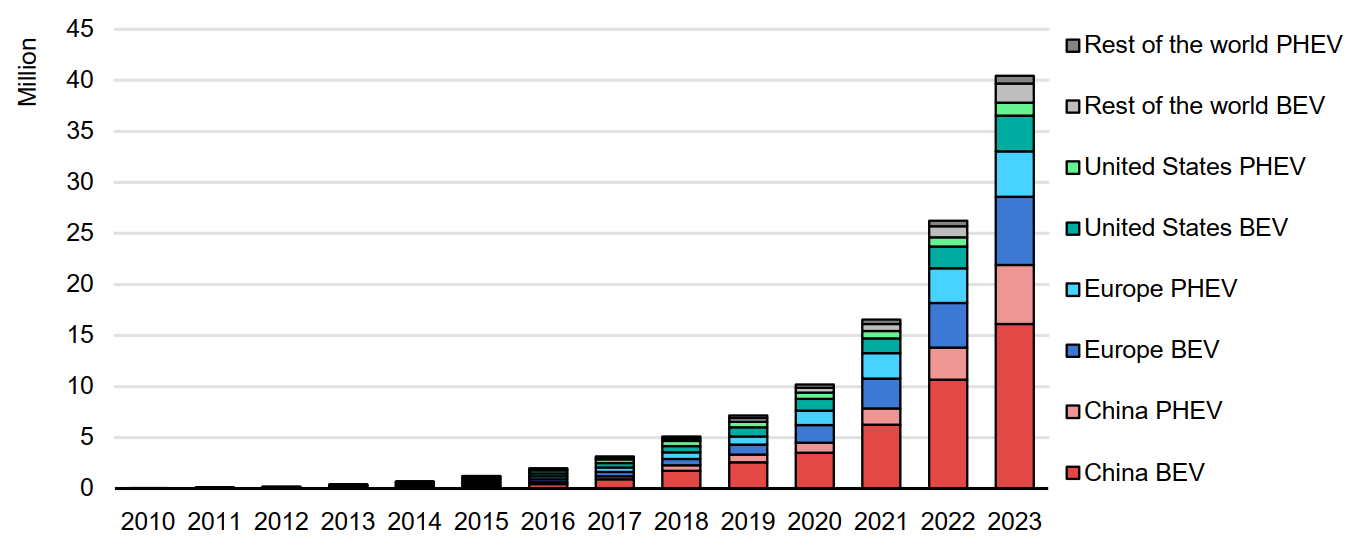
\includegraphics[width=1\textwidth]{FIGURES/Chapter 3/Global electric car stock trends, 2010-2023.png}
    \caption{Global electric car stock trends, 2010-2023}
    \label{fig:EV sale}
\end{figure}

The growing number of EVs worldwide will demand more electricity, leading to a significant rise in their share of total electricity consumption. In 2023, the global EV fleet consumed approximately 130 TWh of electricity, equivalent to Norway’s total electricity demand that year. On a global scale, EVs accounted for about 0.5\% of total final electricity consumption in 2023, with this share rising to around 1\% in China and Europe. The contribution of different EV segments to electricity demand varies by region. For instance, in China in 2023, electric two/three-wheelers and buses together made up nearly 30\% of EV electricity demand, whereas in the United States, electric cars contributed over 95\% of the total EV electricity demand (Fig. \ref{fig:EV demand}) \cite{global_ev_outlook_2024}.

\begin{figure}[h!]
\captionsetup{font=footnotesize}
\captionsetup{justification=centering}
    \centering
    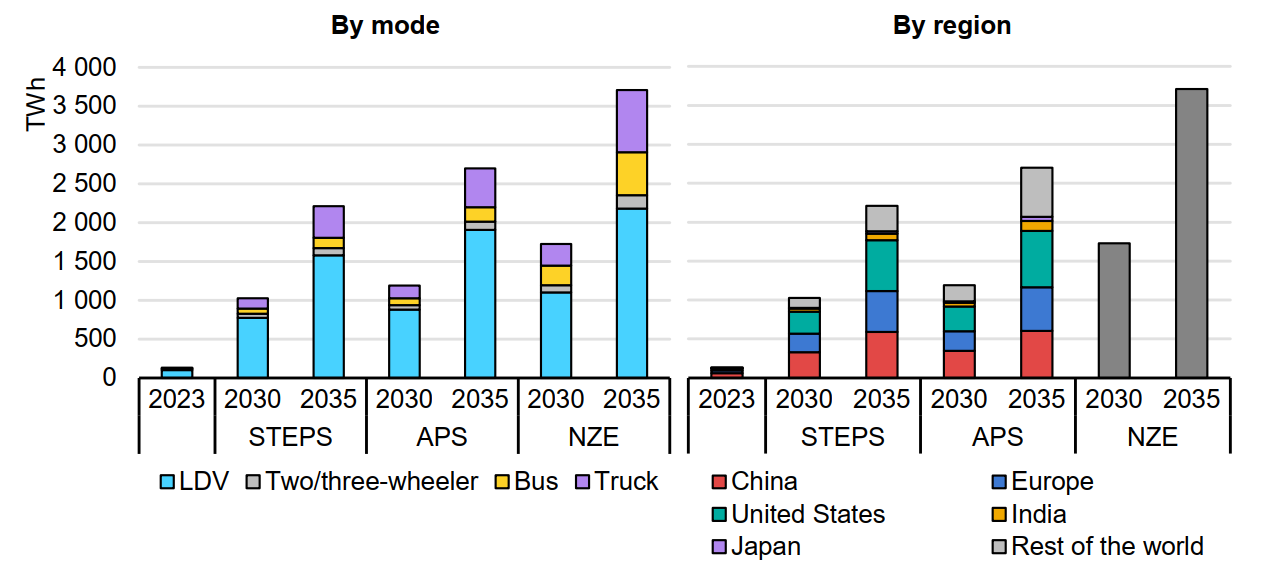
\includegraphics[width=1\textwidth]{FIGURES/Chapter 3/Electricity demand by mode and by region, 2023-2035.png}
    \caption{Electricity demand by mode and by region, 2023-2035}
    \label{fig:EV demand}
\end{figure}


By 2035, EV electricity demand could reach nearly 2,200 TWh in the STEPS and around 2,700 TWh in the APS—over 20\% higher despite only a 15\% increase in EV stock. This disproportionate growth stems from higher electrification rates in markets with greater vehicle mileage, such as the United States, and increased electrification of trucks and buses, which contribute significantly to electricity consumption. In Net-zero pledge countries, a larger share of PHEV mileage is expected to be in full electric mode. Despite accounting for less than 10\% of global final electricity consumption, EVs contribute to overall energy savings due to the higher efficiency of electric powertrains, with total road energy demand in the APS decreasing by 10\% by 2035, even as vehicle activity grows by 20\% (Table \ref{tbl:share of elec}).
\begin{table}[h!]
\centering
\captionsetup{font=footnotesize}
\captionsetup{justification=centering}
\caption{Share of electricity consumption from electric vehicles relative to final electricity consumption by region and scenario, 2023 and 2035}
\small
\begin{tabular}{@{}lccc@{}}
\hline
\toprule
\begin{tabular}[c]{@{}l@{}} \textbf{Country/Region} \end{tabular} &
\begin{tabular}[c]{@{}c@{}} \textbf{2023} \end{tabular} &
\begin{tabular}[c]{@{}c@{}} \textbf{Stated Policies} \\ \textbf{Scenario (2035)}
\end{tabular} &
\begin{tabular}[c]{@{}c@{}} \textbf{Announced
Pledges} \\ \textbf{Scenario (2035)}\end{tabular}
\\ \midrule
China & 0.7 \% & 6.8 \% & 6.9 \% \\ \midrule
Europe & 1.1 \% & 13.7 \% & 14.5 \% \\ \midrule
United States & 0.6 \% & 14.2 \% & 15.6 \% \\ \midrule
Japan & 0.1 \% & 3.1 \% & 5.5 \% \\ \midrule
India & 0.2 \% & 6.0 \% & 8.7 \% \\ \midrule
Global & 0.5 \% & 8.1 \% & 9.8 \% 
\\ \bottomrule
\end{tabular}
\label{tbl:share of elec}
\end{table}
This led to several negative impacts on the grid in terms of power quality, load profile, voltage, etc. Specifically:

\subsection{Voltage}
Voltage stability refers to the ability to maintain steady voltage levels at various nodes in the power system under normal operating conditions. With the increasing load from EV charging, grid voltage stability can be affected, resulting in voltage deviations beyond permissible limits \cite{53_greenin}. The impact of EVs on grid voltage depends on the distribution of EV charging loads across different locations within the grid.

When EVs are charged at nodes near substations, the charging load typically causes minimal voltage deviations at other grid nodes. Conversely, charging EVs at locations far from substations significantly affects voltage drop across the grid \cite{53_greenin}. For example, a study \cite{54_greenin} modeled a 10-node power grid to assess the impact of EV charging location. The results showed that voltage at Node 10 decreased by 3.75\% compared to the substation voltage, leading to a noticeable voltage drop along the feeder. In scenarios where substations are placed at both ends of the feeder, the worst-case scenario occurred when EVs were charged in the middle of the feeder, causing voltage to drop by 1.34\%.

Additionally, the penetration level of EVs is a critical factor influencing voltage stability. Higher EV penetration levels can push voltage levels on the feeder to approach or exceed the lower permissible voltage limit \cite{55_greenin}. A model to determine the maximum EV penetration that does not severely impact grid performance was proposed in \cite{56_greenin}. This study evaluated various EV penetration levels in uncontrolled charging scenarios under two distinct load distribution cases. In Scenario A, voltage violations were not observed as long as the EV penetration rate did not exceed 50\%. However, increasing the penetration rate by an additional 10\% caused voltage to surpass permissible limits in urban grids. In Scenario B, where EV charging loads were unevenly distributed across phases, voltage limits were exceeded at an EV penetration rate of just 25\%. This highlights the importance of balanced EV load distribution to maintain grid stability.

\subsection{Load profile}
The charging demand of electric vehicles (EVs) represents a unique type of load as it is heavily dependent on the behavior and intentions of vehicle owners. In the absence of any restrictions governing EV charging schedules, vehicle owners tend to charge their EVs immediately upon arriving at workplaces or returning home in the evening—coinciding with peak load periods during rush hours \cite{57_greenin,58_greenin}. Numerous studies have been conducted to assess the impact of EV charging on load profiles. For instance, \cite{59_greenin} analyzed EV charging loads in the United Kingdom with varying numbers of EVs, revealing that when the number of EVs requiring charging exceeded 1 million, the daily peak load increased by 3.69\%. Similarly, \cite{60_greenin} predicted the EV charging demand in Germany for the year 2030. In a scenario where all vehicles are replaced with EVs, the energy demand from EVs is projected to raise the peak load to 38.4 GW, a 92\% increase compared to scenarios without EV charging.

Additionally, the charging power levels chosen for EVs significantly influence the overall load profile. In \cite{61_greenin}, the peak loads of two charging modes, Level 1 and Level 2, with charging powers of 1.92 kW and 6.6 kW, respectively, were compared. When EVs accounted for only 3\% of the total vehicle market share, the difference in peak load between the two modes was merely 9 W. However, when the market share of EVs reached 100\%, the difference in peak load increased significantly to 657 W. 

\subsection{Utility grid infrastructure}
Transformers, transmission lines, and switching and protective devices are critical components of the power grid, with transformers being regarded as the most important due to their high repair and replacement costs \cite{62_greenin}. The increasing number of EVs requiring charging not only impacts the load profile but also directly reduces the operational lifespan of transformers. Continuous EV charging can lead to thermal overloading of transformers \cite{63_greenin, 64_greenin, 65_greenin}, thereby decreasing their efficiency and shortening their lifespan. The impact of EV penetration on transformers was analyzed in \cite{64_greenin}, which evaluated three key factors influencing transformer lifespan: temperature, aging rate, and the Loss of Life (LOL) factor. The study concluded that transformers could operate effectively with an EV market share of up to 50\%. However, \cite{65_greenin} compared the LOL factor for both fast and slow charging modes, finding that even with fewer EVs, fast charging resulted in a higher LOL factor. Similarly, \cite{63_greenin} not only reached comparable conclusions but also analyzed transformer temperatures, highlighting the negative impact of fast charging. As a result, researchers recommend fast charging only when necessary, while avoiding high-power charging when vehicles are plugged in for extended periods, such as during work hours.

Such adverse effects have prompted researchers to evaluate the future readiness of power grid infrastructure as EV penetration increases. For instance, with a projected EV market share in Singapore by 2050 utilizing single-phase and three-phase charging, the impact on transformers is expected to remain manageable \cite{66_greenin}. Conversely, Norway's distribution network has been estimated to handle only up to 20\% EV penetration without causing overloads on distribution lines \cite{67_greenin}. In Toronto, EV chargers with power ratings of 3.3 kW or lower are unlikely to negatively affect the grid. However, chargers rated at 10 kW would necessitate infrastructure upgrades to prevent potential issues such as fires and grid overloads \cite{68_greenin}. 

\subsection{Power loss}
Energy loss can be calculated using the formula:
\begin{equation}
    P = I^2 \cdot R
\end{equation}
where $I$ is the current flowing inside the lines in Ampere ($A$), $R$ is the line resistor in Ohm ($\Omega$).

As the number of EVs being charged increases, the demand for electricity for charging purposes rises, leading to greater power flows across the system and, consequently, higher power losses \cite{69_greenin}. In \cite{70_greenin}, the level of power losses was calculated to establish the relationship between grid power losses and the number of EVs being charged. The study concluded that when EVs constitute the majority of vehicles integrated into the grid—62\% of all vehicles on the road—power losses can reach up to 40\% during off-peak hours, as most vehicles are charged at this time. EV charging in residential areas can significantly exacerbate power losses in transformers. According to \cite{71_greenin}, when EV penetration reaches 40\%, power losses in transformers could triple their rated capacity.

Several studies have been published to evaluate power losses on the grids of different countries. Research \cite{72_greenin} calculated energy losses based on real-world distribution grid data in Denmark. When EV penetration reached 50\%, power losses increased by 40\%. Similarly, \cite{73_greenin} assessed power losses in low-voltage networks in Denton East, UK, under various EV penetration levels. The study showed that as EV penetration increased, real power losses also rose, with losses reaching nearly 50 kW when 90\% of vehicles were EVs.

\subsection{Harmonic}
Harmonics are waveforms whose frequencies are integer multiples of the fundamental frequency \cite{74_greenin}, typically generated by nonlinear loads such as EV chargers and other similar devices. Harmonics are quantified using Total Harmonic Distortion (THD) \cite{75_greenin}. Specifically, the voltage Total Harmonic Distortion is defined as the ratio of the root mean square (RMS) value of the harmonic components of the voltage to the RMS value of the fundamental voltage component \cite{76_greenin}, as described by Equation \eqref{eqt:THD}:
\begin{equation}
    THD = \sqrt{\frac{\sum_{h=2}^{H} V_h^2}{V_{grid}^2}} \times 100\%
    \label{eqt:THD}
\end{equation}
where: 
\begin{itemize}
    \item THD: Total Harmonic Distortion
    \item $V_h$: The root mean square (RMS) value of the voltage harmonic at the $h^{th}$ order, where $H$ represents the highest order of harmonics under evaluation
    \item $V_{grid}$: The RMS value of the grid fundamental voltage component (at a frequency of 50 Hz)
\end{itemize}

The Circular No. 39/2015/TT-BCT issued by the Ministry of Industry and Trade of Vietnam regarding the distribution power system in Vietnam stipulates about the THD and Individual Distortion as in Table \ref{tbl:TT-BCT} \cite{76_greenin}.
\begin{table}[h!]
\centering
\captionsetup{font=footnotesize}
\captionsetup{justification=centering}
\caption{Regulations regarding Total Harmonic Distortion (THD) and individual harmonic distortion in Vietnam}
\small
\begin{tabular}{@{}lcc@{}}
\hline
\toprule
\begin{tabular}[c]{@{}l@{}} \textbf{Voltage Level} \end{tabular} &
\begin{tabular}[c]{@{}c@{}} \textbf{Total Harmonic Distortion} \\ \textit{\textbf{(THD)}} \end{tabular} &
\begin{tabular}[c]{@{}c@{}} \textbf{Individual Distortion} \\ 
\end{tabular} 
\\ \midrule
110 kV & 3.0 \% & 1.5 \% \\ \midrule
Medium \& Low Voltage & 6.5 \% & 3.0 \% 
\\ \bottomrule
\end{tabular}
\label{tbl:TT-BCT}
\end{table}

Due to the nonlinear characteristics of Electric Vehicle (EV) loads, studies evaluating the impact of EV charging loads on power quality in terms of harmonic distortion are necessary. Research \cite{77_greenin} assessed the impact of EV loads under both light and heavy load conditions based on the IEC 61000 and EN 50160 standards. In scenarios where the load for other electrical demands is low, when the total harmonic distortion (THD) of the current reaches 5.6\%, the THD of the voltage does not exceed the threshold limit. However, the opposite scenario occurs when the load is high: the voltage THD exceeds the 8\% limit when EVs account for a large portion of the total number of vehicles. From this, it can be inferred that a significant number of EVs being charged would notably affect the distribution grid by causing substantial harmonic distortion \cite{78_greenin, 79_greenin}. A similar conclusion was found in research \cite{80_greenin}, which examined the harmonic impact of loads on the power grid in Bangladesh, concluding based on the IEEE Standard 519-2014. The current number of EVs in Bangladesh is still modest and does not pose a significant concern for the grid. However, with a forecasted increase in the number of EVs, the voltage THD may exceed allowable limits. In article \cite{81_greenin}, it was concluded that EVs charged at higher state-of-charge (SOC) levels would have less of a concerning impact on the power grid as well as on the EV battery.

\subsection{Frequency}
Frequency is a critical factor influencing the operation of the electrical system. According to Decree No. 137/2013/ND-CP \cite{82_greenin}, under normal conditions, the permissible frequency deviation of the power system is within ± 0.2 Hz from the nominal frequency of 50 Hz. A frequency deviation exceeding the allowable limits can cause equipment malfunctions, fires, and explosions, as well as system failures such as power outages and short circuits. Research \cite{83_greenin} has shown the impact of EV loads on the frequency of the power grid. In a scenario where only EVs are present, the frequency at certain times drops below 49.5 Hz, surpassing the permissible frequency limits. When combined with renewable energy sources such as photovoltaic (PV) systems, the impact on the grid frequency increases. Specifically, if vehicles do not control the charging process, the grid frequency at certain times may exceed 50.5 Hz, potentially reaching nearly 51 Hz.

To accurately assess the negative impact of EV loads on the power grid, it is necessary to consider other factors in the EV charging process. Article \cite{84_greenin} analyzed factors such as the charging method and the level of EV penetration on grid frequency. With respect to the charging method, it was observed that charging without grid support causes the frequency to drop to nearly 49.8 Hz. The study also simulated the potential impacts based on the projected number of EVs expected by 2050. In all cases considered, when EVs charge without supporting the grid frequency, it creates a negative impact, with the minimum frequency only reaching 49.82 Hz. Conversely, in other cases, the lowest achievable frequency was around 49.88 Hz.

%%-------------------------------------------------------%%
% --------------------------------------------------------%
%---------------------------------------------------------%


\newpage
%% --------------------------------------------------%%
%------------ CHAPTER 4 ---------------------------%
%%-----------------------------------------------------%
\section*{CHAPTER 4. STRATEGIES AND SOLUTIONS TO MITIGATE THE EFFECTS OF EVS ON THE POWER GRID}

   \label{chuong4}
    \addcontentsline{toc}{section}{\numberline{}CHAPTER 4. STRATEGIES AND SOLUTIONS TO MITIGATE THE EFFECTS OF EVS ON THE POWER GRID}
    
\setcounter{section}{4}
    \setcounter{subsection}{0}
        \setcounter{figure}{0}
            \setcounter{table}{0}
\sloppy
%--------------------------------------------------------%

To meet the growing energy demand driven by the increasing adoption of electric vehicles (EVs), the deployment of public EV charging stations (EVCSs) must keep pace. However, poorly planned EVCS infrastructure can adversely affect profitability for stakeholders and also lead to inefficiency in resource utilization. If the number of charging stations is insufficient to meet the aggregate charging demand, it can lead to congestion with waiting queues and potential overload of the EVCSs, particularly in areas with a high density of EVs per capita. Conversely, if the total capacity of charging stations greatly exceeds the demand, it will directly impact station owners due to the low utilization of charging facilities, resulting in diminished profits and wasteful expenditure of land, energy, and capital resources. An unbalanced ratio of EVCS to EVs might not facilitate a user-friendly experience and can even deter potential EV adopters. Furthermore, the location of EVCSs also has to be carefully planned for easy access by users and to ensure sufficient energy supply for a given area.

To optimize the construction and operation of EVCSs, it is required that the benefits for all agents are balanced. For the charging station owner, the objective is to maximize the return on investment of their EVCS. For the grid aggregator, grid stability, power loss, and other parameters must remain within acceptable limits. For EV owners, the key requirements are minimizing the cost of recharging their vehicle batteries and ensuring convenient access to charging services. Besides these objectives, which need optimization for best results, there are various constraints that must be followed, from the construction of an EVCS to its operation.

Researches have been made to address one or more objectives simultaneously, from the perspective of each individuals: 

\begin{itemize}
    \item \textit{i. For grid aggregator:} Study \cite{86_greenin} optimized EV charging station locations in a 30-node grid (21 load nodes, 14 stations) in Allahabad, India, using the Balanced Mayfly Algorithm (BMA). BMA outperformed two other algorithms, effectively minimizing reactive and active power losses, infrastructure upgrade costs, and finding the optimal location of the charging station and their numbers. Similarly, \cite{87_greenin} presented a multi-objective (MO) strategy for microgrids, targeting both reduced peak load, which resulted in a decrease of nearly 10kW, and improved voltage profiles. The results show that the voltage values were optimized with controlled charging strategies. This resulted in optimized location and number of charging points and improvements in power loss and voltage values in both researches. A mixed step-size normalized least mean fourth control algorithm is suggested in \cite{Balasundar2022}. This algorithm, implemented with bidirectional AC-DC and DC-DC converters, a distribution static compensator, and a Li-ion battery, regulates voltage and minimizes harmonic distortion in the electrical grid, maintaining operation within required standards. In paper \cite{li2019mpc} they use a model predictive model (MPC) allow EVs to participate in grid voltage regulation as reactive power compensation devices, through a two-stage hierarchical control scheme. By that, the voltage deviations from the nominal value is minimized simultaneously with EV being charged to the desired SOC without violating any grid constraints. Power smoothing can be effectively achieved by integrating renewable energy sources (RES) and battery energy storage systems (BESS) into EVCS. Renewable generations, particularly from photovoltaic (PV) and wind systems, offers non-emission and cost-effective solutions \cite{RES}. Study \cite{Zhiyong2020} shows that rooftop PV integrated EVCSs with vehicle-to-grid technology reduce peak load and operating costs compared to schemes without PV and improve energy efficiency.
    \item \textit{ii. For EVCS owners:} Renewables and BESS continue to support the stakeholders of the EVCS with proper configuration and management. A research \cite{MMOSSA} offers a novel Modified Multi-objective Salp Swarm Optimization Algorithm (MMOSSA)-based technique for optimal photovoltaic (PV), wind turbine (WT), BESS-VSG (Virtual Synchronous Generator), and EVCS allocation on microgrids, to achieve multi objectives of total net present cost (NPV), levelized cost of energy (LCOE), energy loss, frequency deviation, voltage stability, and carbon emissions. It has effectively increase total NPV, reduced LCOE and emissions with this configuration, in 2 conflicting environment and EV charging patterns, and all of the technical constraints are significantly improved. In paper \cite{Sun2020}, a hybrid optimization approach combining MOPSO and TOPSIS was proposed to minimize both energy costs and GHG emissions. The scenario analysis concludes that the combination of renewable energy supplies, the connection with utility grid and DR can help improve the performance on optimization objectives. 
    \item \textit{iii. For EV owners:} Study \cite{88_greenin} explored the optimal placement of fast charging stations, aiming to minimize charging wait times and maximize station utilization using a binary search algorithm. With the optimized locations, most vehicles would experience wait times under 10 minutes. Additionally, node voltages were maintained within the range of 0.95 ($V_{min}$) to 1.05 ($V_{max}$). Researchers in \cite{moghaddam2017smart} proposes a smart charging strategy for PEV networks, offering multiple charging options with varied capacities and pricing. They model this as a multi-objective optimization problem minimizing charging time, travel time, and cost, and use a queuing model to estimate delays. Partial charging is introduced to mitigate peak load overlap. The results show a 25\% reduction in average charging delay and 15\% cost reduction.
\end{itemize}

Beside these technology, which mainly about uni-directional V1G charging technology, Vehicle-to-Grid (V2G) is also an effective solution, not only reducing impacts on the grid but also improving the power quality of the grid \cite{91_greenin}. Paper \cite{92_greenin} employed a V2G optimization algorithm, reducing the peak-to-valley load difference from 5 MW to 1.5 MW. V2G also provides economic benefits for EV owners by enabling them to earn revenue through grid discharge, thus offsetting charging costs. Study \cite{94_greenin} used a linear programming algorithm to optimize both operator and owner profits, improving grid operator profits by 113\% and reducing EV charging costs by 17.4\%. Study \cite{95_greenin} proposed a V2G optimized by the Water Cycle Algorithm (WCA) to address EV charging prices. A comparison of charging prices in V2G/G2V and G2V scenarios shows a positive correlation between the price difference and the number of EVs.
\clearpage

%%-------------------------------------------------------%%
% --------------------------------------------------------%
%---------------------------------------------------------%

%% CONCLUSIONS
\section*{CHAPTER 5. CONCLUSION}
   \label{chuong5}
    \addcontentsline{toc}{section}{\numberline{}CHAPTER 5. CONCLUSION}
    
\setcounter{section}{5}
    \setcounter{subsection}{0}
        \setcounter{figure}{0}
            \setcounter{table}{0}
%%-------------------------------------------------------%%
% --------------------------------------------------------%
%---------------------------------------------------------%

The report has an overview of related facets related to EV charging. Different EV charging technologies and their standards in \textbf{Chapter 2}, negative impacts of EV charging to the grid in \textbf{Chapter 3} and some of the solutions to mitigate them in \textbf{Chapter 4}. The most significant conclusions can be outlined as follows:
\begin{itemize}
    \item Beside conductive charging being the most mature, EV can also be charged by wireless or by battery swap scheme, however they still need more experiments in real life
    \item EV charging can heavily affect the quality of the utility grid, thus there is a need to control the charging protocol and design a proper EVCS
    \item Different strategies is used to minimize not only the negative impacts of charging EVs on the grid, but also to maximize profit for other agents, such as the EVCS owner or to the station customers
    \item EVCS with renewable energy and BESS integrated can significantly improved the grid quality if being properly sized and controlled
    \item The role of EVs are not only the load that consume power, but they can also act as a source of energy via V2G, which can support the grid
\end{itemize}

Beside advancements in Vehicle-to-Grid (V1G) technology, EV owners still have doubts and concerns regarding Vehicle-to-Grid (V2G) implementation. These concerns primarily stem from fears of cybersecurity attacks, a lack of privacy, and the potential impact of densely charging and discharging sequences on their EV battery pack's health. Fostering public acceptance requires ensuring user privacy and offering tangible rewards for participation in grid-discharge programs. In the future, integrating multiple strategies can simultaneously optimize various objectives. Furthermore, developments in PV, wind turbine, and BESS technologies will likely reduce costs, making hybrid EVCSs that combine renewable sources with energy storage systems more feasible and appealing to stakeholders. EV users will also benefit from this trend as the levelized cost of energy (LCOE) is expected to decrease.

\newpage
% REFERENCES
\phantomsection\addcontentsline{toc}{section}{\numberline {}REFERENCES}

\bibliography{citation}
\newpage

% APPENDIX
%\section*{PHỤ LỤC}
 %   \phantomsection\addcontentsline{toc}{section}{\numberline{} PHỤ LỤC}

%Phụ lục cần thêm (nếu có)
%...
\newpage
\thispagestyle{empty}
\end{document}